\section{Introduction}
\label{sec:introduction}

Graphics processing units (GPUs) are becoming powerful many-core compute
devices.
For example, NVIDIA GPUs integrate more than $1,500$ processing cores on
a single chip and the peak double-precision performance exceeds 1
TFLOPS while sustaining thermal design power (TDP) in the same order of
magnitude as traditional multicore CPUs~\cite{NVIDIA_Kepler}. 
This rapid growth of GPUs is due to recent advances in the
programming model, often referred to as general-purpose computing on
GPUs (GPGPU).

Data-parallel and compute-intensive applications receive significant
performance benefits from GPGPU.
Currently a main application of GPGPU is supercomputing~\cite{TOP500}
but there are more and more emerging applications in different fields.
Examples include plasma control~\cite{Kato_ICCPS13}, autonomous
driving~\cite{McNaughton_ICRA11}, software routing~\cite{Han_SIGCOMM10},
encrypted networking~\cite{Jang_NSDI11}, and storage
management~\cite{Bhatotia_FAST12, Gharaibeh_HPDC10, Kato_ATC12,
Sun_SYSTOR12}.
This broad range of applications raises the need of further developing
GPU technology to enhance scalability of emerging data-parallel and
compute-intensive applications.

Grand challenges of GPU computing include an integration of real-time
systems.
So far the real-time systems community has addressed resource management
issues for GPUs~\cite{Basaran_ECRTS12, Elliott_RTS12, Elliott_ECRTS12,
Kato_ATC11, Kato_RTAS11, Kato_RTSS11}, but the main contribution of
these work is limited to the scheduling of compute kernels and data
transfers.
The basic performance and latency issues for GPUs are not well studied
in the literature.
Given that compute kernels are offloaded to the GPU, their performance
and latency are more dominated by compiler and hardware technology.
However an optimization of data transfers must be complemented by system
software due to the constraint of PCIe devices~\cite{Kato_ATC12}.
Data transfers may also be interfered by competing workload on the CPU,
while offloaded compute kernels are isolated on the GPU.
These data transfer issues must be well understood and addressed to
build predictable soft real-time systems, if not hard real-time systems,
being integrated with cutting-edge GPU technology.

The data transfer is particularly an important issue for low-latency GPU
computing.
Kato~\textit{et. al.} demonstrated that the data transfer is a dominant
property of GPU-accelerated plasma control systems~\cite{Kato_ICCPS13}.
This is a specific application where the data must be transferred
between sensor/actuator devices and the GPU at a high-rate, but is a
good example presenting impact of data transfers for GPU computing.
Since emerging applications augmented with GPUs may demand a similar
performance requirement, a better understanding of the GPU data transfer
mechanism is desired.

\begin{figure}[!t]
 \centering
 \subfigure[Host to Device]{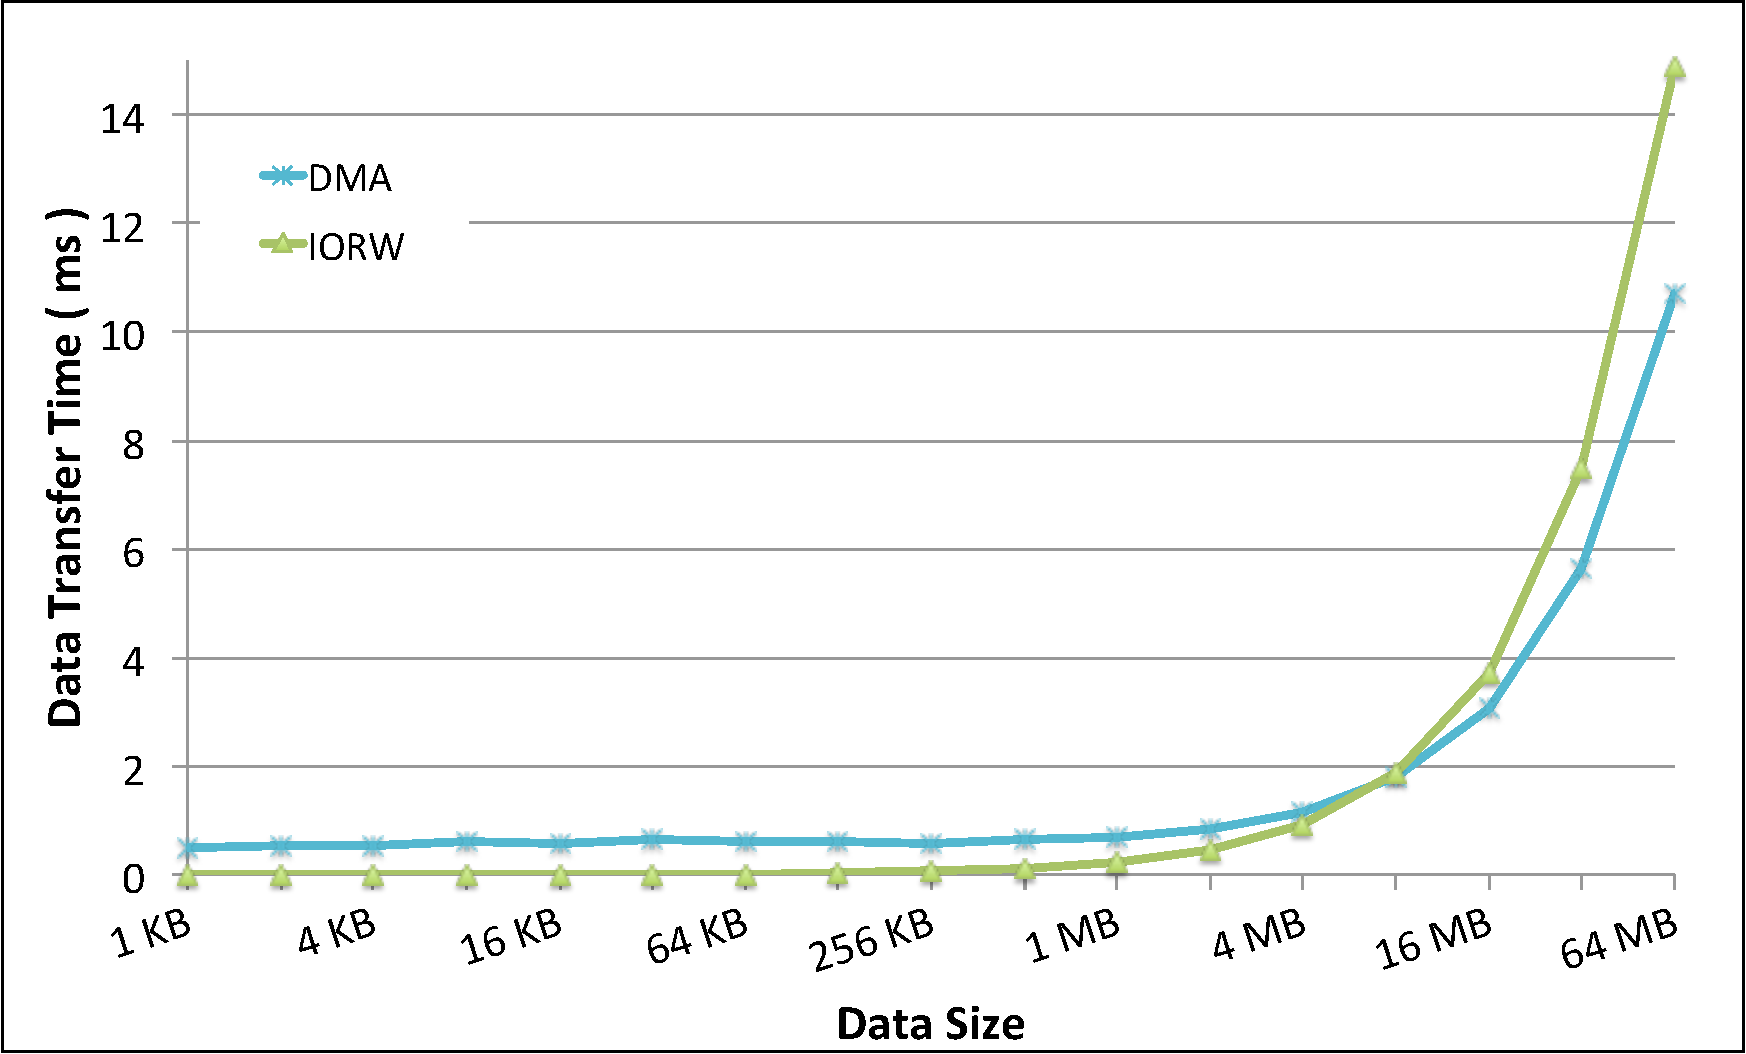
\includegraphics[width=0.33\textwidth]{figure/Graph/forIntro_HtoD.pdf}}\\
 \subfigure[Device to Host]{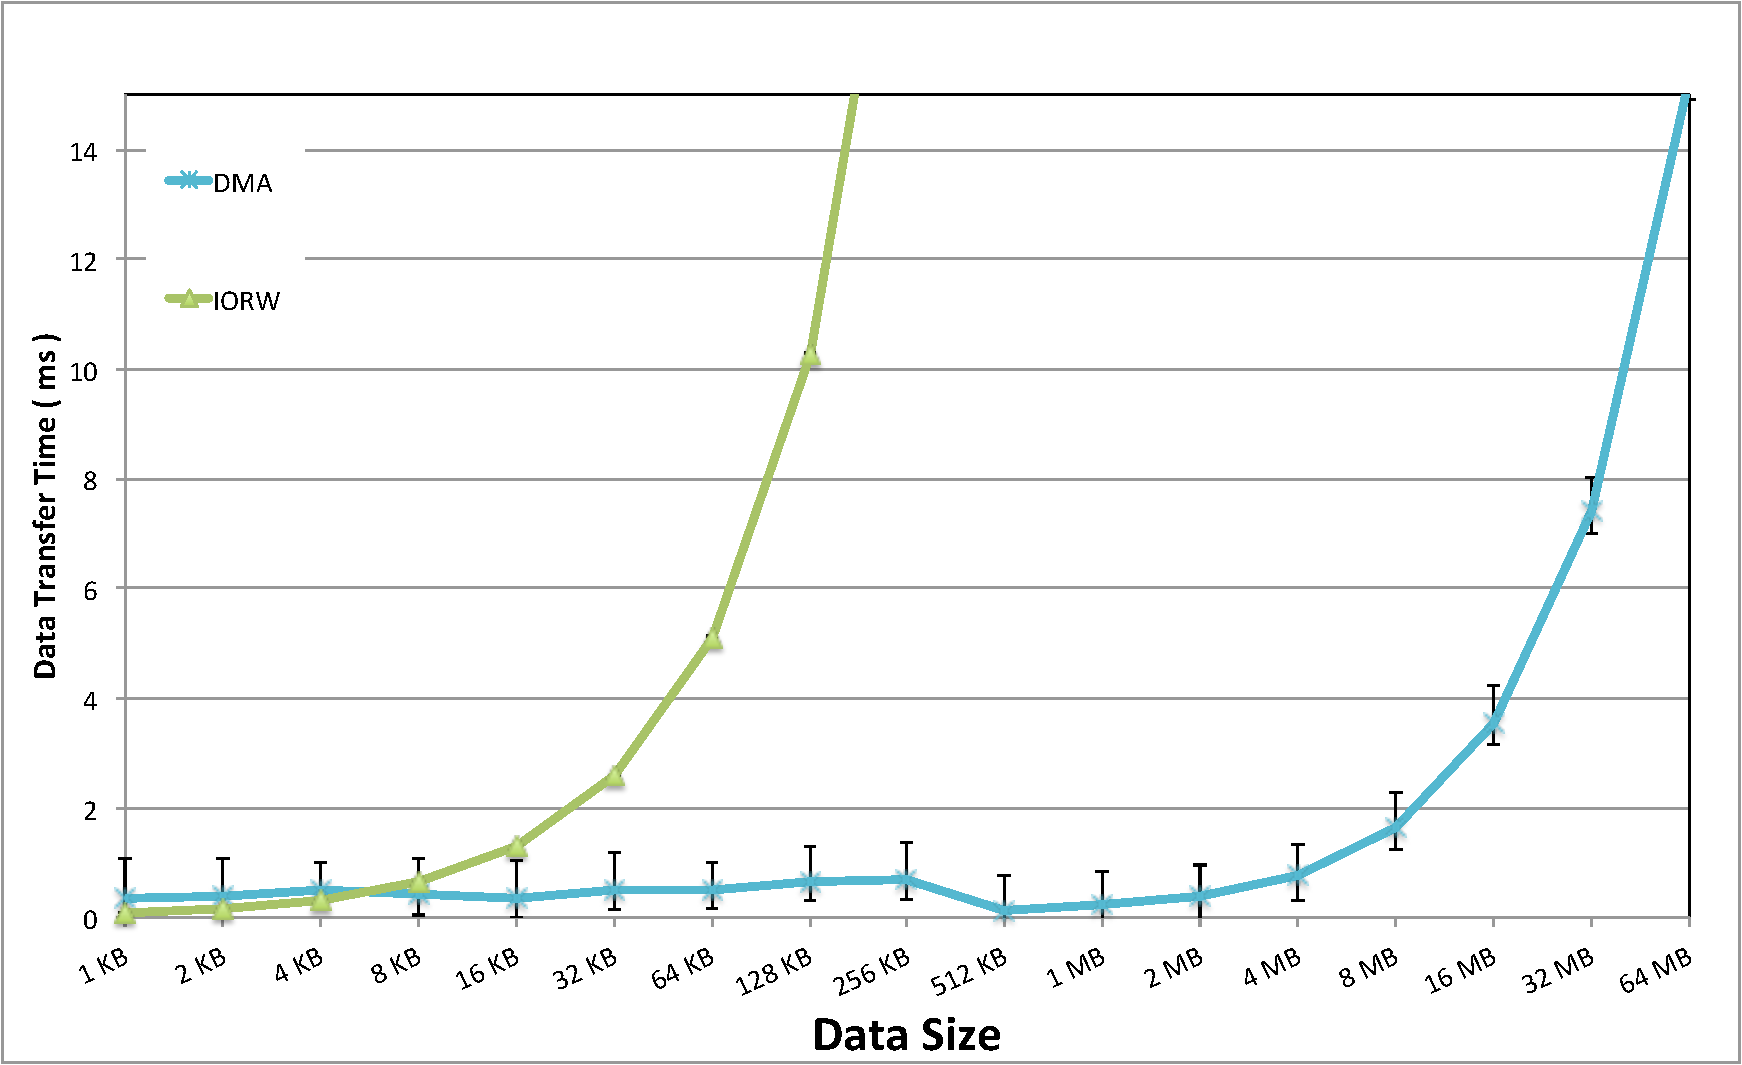
\includegraphics[width=0.33\textwidth]{figure/Graph/forIntro_DtoH.pdf}}
 \caption{Performance of DMA and I/O read/write for the NVIDIA GPU.}
 \label{fig:intro_data_transfer}
\end{figure}

Figure~\ref{fig:intro_data_transfer} depicts the average data transfer
times of hardware-based direct memory access (DMA) and memory-mapped I/O
read-and-write access, which are obtained on an NVIDIA GeForce GTX~480
graphics card using the open-source Linux driver~\cite{Kato_ATC12}.
Apparently the performance characteristics of the data transfer are not
identical for the host-to-device and device-to-host directions.
In previous work, a very elementary issue of this performance difference
has been discussed~\cite{Kato_ATC12}, but there is no clear conclusion
on what methods can optimize the data transfer performance, what
different methods are available, and what is their implication for
real-time systems.
Currently we pray that the black-box data transfer mechanism of
proprietary software, provided by GPU vendors, is well optimized to
meet the performance that programmers expect, because hardware details
of GPUs are not disclosed to the public.
However real-time systems must build on a predictable basis.
We must understand what latency and performance interference exist when
using the GPU.
To some extent the GPU is suitable for predictability once the workload
is offloaded, but associated data transfers may compete with the
host computer workload.
Hence a better understanding of the data transfer relevant to GPU
computing is an essential piece of work to support real-time systems
with GPUs.
Unfortunately prior work~\cite{Kato_ATC12, Kato_ICCPS13} did not provide
performance characterization in the context of real-time and
concurrent workload; they focused on a basic comparison of DMA and
direct I/O access.

\textbf{Contribution:}
In this paper, we clarify the performance characteristics of
currently-achievable data transfer methods for GPU computing while
unveiling several new data transfer methods other than the well-known
DMA and I/O read-and-write access.
We reveal the advantage and disadvantage of these methods in a
quantitative way leading a conclusion that the typical DMA and I/O
read-and-write methods are the most effective in latency even in the
presence of compelling workload, whereas concurrent data streams from
multiple different contexts can benefit from the capability of on-chip
microcontrollers integrated in the GPU.
To the best of our knowledge, this is the first evidence of data
transfer matters for GPU computing beyond an intuitive expectation,
which allows system designers to choose appropriate data transfer
methods depending on the requirement of their latency-sensitive GPU
applications.
Without our findings, none can reason about the usage of GPUs minimizing
the data transfer latency and performance interference.
Given that the contribution of this paper is not limited to a specific
GPU but is applicable for PCIe compute devices, it is significant for a
grander vision of high-performance real-time systems with GPUs and
future heterogeneous architectures.

\textbf{Organization:}
The rest of this paper is organized as follows.
Section~\ref{sec:assumption} presents the assumption and terminology
behind this paper.
Section~\ref{sec:data_transfer_methods} provides an open investigation
of data transfer methods for GPU computing.
Section~\ref{sec:empirical_comparison} compares the performances of the
investigated data transfer methods in the context of real-time systems.
Related work are discussed in Section~\ref{sec:related_work}.
We provide our concluding remarks in Section~\ref{sec:conclusion}.
